% Chapter 1

\chapter{Introduction} % Main chapter title

\label{Chapter1} % For referencing the chapter elsewhere, use \ref{Chapter1} 

\textbf{Summary}: \emph{This chapter...}

\textbf{R\'esum\'e}: \emph{Cette chapitre...}

% \lhead{Chapter 1. \emph{Introduction}} % This is for the header on each page - perhaps a shortened title

%----------------------------------------------------------------------------------------

\section{Computational phenotyping}

The success of the Human Genome Project (\cite{lander2001initial}) in mapping the totality of human genes has inspired similar efforts for the enumeration of biological phenotypes. An organism's phenotype is the sum of its observable characteristics, encompassing the internal, such as cellular and tissular components, and the external characteristics, such as morphology and behaviour. To be sure, an organism's \emph{phenome} is vastly more high dimensional than the genome, of which, along with external environmental factors it is a function, and is moreover generally not fixed in time as the genetic code is (\cite{houle2010phenomics}). Phenotypes are more intelligible units of measurement than genes for important biological outcomes, natural selection is considered to operate in the ``P-space'' of possible phenotypes, with selection propagating to the ``G-space'' of possible genotypes.

The interest in \emph{phenomics} (by analogy to \emph{genomics}) coincides with the rise of bioimage informatics (\cite{myers2012bioimage}). Bioimages, deriving from the various forms of microscopy, contain rich information on the morphological aspects of cells, cell populations in culture, and tissue histopathological data, and complete organisms, that is lost in other biological readouts. Bioimages in time-lapse can additionally reveal behaviour and track phenotypic changes in motion. Thus, bioimages are a favoured medium for phenotypic information.

\subsection{High content screening}
\label{subsec:hcs}

HCS is the extension of HTS to the imaging domain

High content screening (HCS) is an apt methodology for the systematic discovery of phenotypes from image data, sitting at the nexus of high content analysis (HCA) and high throughput screening (HTS). HCS can be used for fundamental biological research, where gene expression can be modulated via techniques such as RNA interference, or otherwise knocked out entirely, inducing phenotypic effects in cultured cells (see, for example, \cite{neumann2010phenotypic}). HCS also plays a role in the early ``hit-to-lead'' stages of the drug discovery process (\cite{haney2006high}, \cite{pepperkok2006high}). In a typical HCS assay a cell line population is exposed to \emph{small molecule} drug compounds. HCS for drug screening is the subject of Part \ref{partI} of this dissertation. Part \ref{partII}, though not strictly based on a screen, employs high content analysis and shares many characteristics.

The term \emph{high content} refers to the multiplicity of measurements or \emph{readouts} taken for each cell, whose composite constitutes a complex phenotype, in contrast with HTS, which normally screens for a more simple output. Most often, these measurements derive from the various channels of fluorescence microscopy imagery. Fluorescence microscopy uses a laser to excite fluorescent molecules in organic matter. These molecules are known as \emph{fluorophores}. In HCS, cells are exposed to fluorescent stains so as to highlight key regions. The fluorescent stains are selected in accordance with the research questions. The subject of analysis of an HCS assay is an immortalised cell line, (hereafter referred to as a \emph{cell line}), which consists in a population of cells, sustained by division without senescence. In this way, a cell line continues replicating indefinitely from a common ancestor. The first and most well-known cell line generated is the HeLa cell line \cite{scherer1953studies}. Since HeLa, many cell lines have been developed. A cell line is thus the model for a disease. Cell lines are useful biological models due to their longevity in cell culture, and are used extensively in biomedical research, for example in assessing the cytotoxicity of a drug treatment. However, their accuracy as biological models can be compromised by their nature as mutated cells, and the effects of repeated passages, cloning, and biochemical contaminants can lead to significant genetic drift from their \emph{in vivo} ancestors (\cite{marx2014cell}). This is one motivation for a multi-cell line screen. In Part \ref{partI} of this disseration, we study multiple triple negative breast cancer (TNBC) cell lines. In Part \ref{partII} we study the Raji cell line as a model for lymphoma. Further details can be found in the relevant chapters.

\begin{figure}
\centering
\begin{tikzpicture}[every label/.append style={text=black, font=\tiny}]
%\draw[step=1.5,thick] (0,-6) grid (6,0);
%\draw[use as bounding box, transparent] (0, 0) rectangle (10, 8);
\filldraw[fill=white, line width=0.3mm](0, 0) -- (0, 4.7) -- (6.8, 4.7) -- (6.8, 0) -- (0, 0);
\filldraw[fill={rgb,255:red,200; green,200; blue,200}, line width=0.3mm](0.1, 0.2) -- (0.1, 4.5) -- (0.2, 4.6) -- (6.4, 4.6) -- (6.7, 4.3) -- (6.7, 0.4) -- (6.4, 0.1) -- (0.2, 0.1) -- (0.1, 0.2);
\def\d{0.2}
\foreach \x in {1,...,12}
{   \foreach \c [count=\y from 1] in {H, G, F, E, D, C, B, A}
    {
    	\ifnum\y=1
        	\ifnum\x=1
	        	\node[circle,draw=black,fill={rgb,255:red,226;green,224;blue,146},minimum size=10, line width=0.2mm, label=left:{\c}, label=below:{\x}] at (\d+0.5*\x,\d+0.5*\y){};
			\else
        		\node[circle,draw=black,fill={rgb,255:red,226;green,224;blue,146},minimum size=10, line width=0.2mm, label=below:{\x}] at (\d+0.5*\x,\d+0.5*\y) {};
			\fi
        \else
        	\ifnum\x=1
	        	\node[circle,draw=black,fill={rgb,255:red,226;green,224;blue,146},minimum size=10, line width=0.2mm, label=left:{\c}] at (\d+0.5*\x,\d+0.5*\y){};
			\else
				\node[circle,draw=black,fill={rgb,255:red,226;green,224;blue,146},minimum size=10, line width=0.2mm] at (\d+0.5*\x,\d+0.5*\y){};
			\fi
	    \fi

%    	\if\x1
%        \node[circle,draw=black,fill={rgb,255:red,50;green,180;blue,70},minimum size=10, label=left:{\c}] at (0.1+0.5*\x,0.1+0.5*\y) {};
%        \elset
%	        \node[circle,draw=black,fill={rgb,255:red,50;green,180;blue,70},minimum size=10] at (0.5*\x,0.5*\y){};
%	    \fi
    }
}
\draw[line width=0.2mm] (5.7, 3.88) -- (8, 3.8);
\draw[line width=0.2mm] (5.7, 3.52) -- (8, 0.8);

\node[inner sep=0pt, drop shadow, anchor=west] (original) at (8, 2.3) {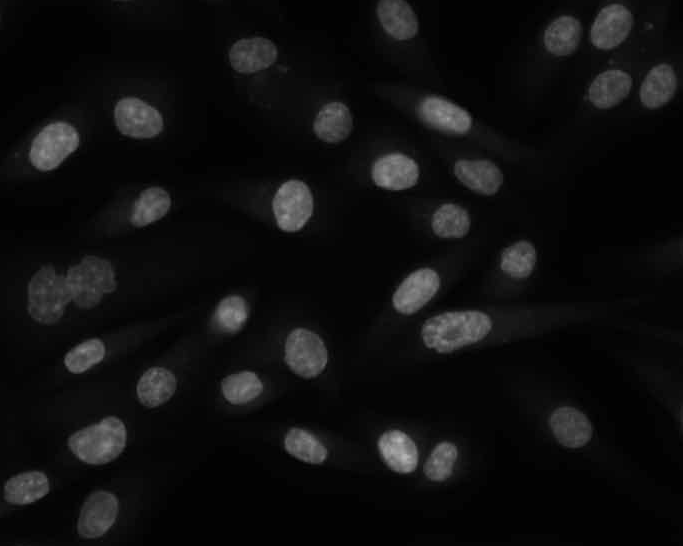
\includegraphics[height=3cm]{img/DAPI_crop}};

\end{tikzpicture}
\caption{Depiction of a 96-well microplate alongside fluorescence (single-channel) image highlighting cell nuclei.}
\label{fig:microplate}
\end{figure}

Each well of a microtiter plate\footnote{Microtiter plates (hereafter \emph{plates}) are small (usually polystyrene) trays divided into a rectangular grid of wells functioning as individual test tubes.} (Figure \ref{fig:microplate}), is seeded to confluence with cells of a chosen cell line. It is favourable to the downstream image analysis to seed cells at a density that will minimise cell overlap. This is because a typical first step in the analysis pipeline is the segmentation of individual cells. The seeding density must therefore be chosen according to the unique morphological properties of the cell line (\cite{bray2016cell}). Within each well, some number of images corresponding to non-overlapping \emph{fields of view} (we henceforth use the term \emph{fields}) are taken, typically producing from hundreds to thousands of unique images per plate.

High throughput screens compare populations of negative controls with others exposed to perturbation. \cite{swinney2011were} differentiate target-based and phenotypic screens. The study looks at 257 drugs published between 1999 and 2008. Despite the preeminence of target-based approaches, they find the most common mode of first-in-class drug discovery is phenotypic screening. This is most true of infectious and central nervous system diseases. Cancer treatments are most frequently discovered by biologics\footnote{Biologics are genetically-engineered proteins that target the immune system.}, which also predominate for diseases of the immune system. Target-based approaches succeed for the discovery of half of the follower drugs. 

A typical HTS project workflow commences with a pilot screen that validates the pipeline from experimental protocol through to image analysis (see \cite{terjung2010high}). This is followed by a large scale screen, increasing the number of perturbations tested. It is here that candidate \emph{hits} are identified. An HTS assay is subject to random variation as well as systematic measurement error. A typical validation step in therefore is to assure statistics measured between controls and test samples can be distinguished with confidence. The \emph{$Z$-factor} (\cite{zhang1999simple}) expresses the ratio of the separation band $|\mu_c - \mu_s| + 3\sigma_c + 3\sigma_s$ (that is, the distance between the opposing tails of the distributions at three standard deviations) and the dynamic range, $|\mu_c - \mu_s|$ between the control $c$ and the test sample $s$. Thus, the Z factor,

\begin{equation}
Z = 1 - \frac{3\sigma_c + 3\sigma_s}{|\mu_c - \mu_s|}
\end{equation}

The maximum (ideal) value is therefore $1$. In the field, it is an accepted fact that anything below $0$ is considered as a readout lacking robustness. The related $Z'$-factor calculates the same statistic for the positive and negative controls. The positive and negative controls should represent the high and low of the range of measurements of a property of interest. The Z'-factor thus refers to the overall quality of the assay.

Finally, candidate hits are carried forward to secondary screens, involving a greater degree of detail. In spite of this idealised workflow, we are restricted in Part \ref{partI} to the pilot phase of a planned larger screen. We nevertheless find ample phenotypes to observe and on which to develop new methods.

%\begin{quote}
%From my perspective, it is very reminiscent of the state of bioinformatics in the early 1980s: the exciting, somewhat chaotic free-for-all that is potentially the birth of something new. 
%\end{quote}
%
%1.1.1 Give first an overview, positioning HCS wrt other technologies HTS, RNAi, mention phenophics, assay development?
%
%defines phenomics (Houle reference), compares to genomics, advocates image analysis for phenomics
%
%compares hcs with hts and advocates hcs as a tool for phenomics
%
%discusses HCS for fundamental research: RNAi up/down-regulated genes and localisation studies
%
%(finally) HCS for drug discovery

%High content screening (HCS) is a pre-clinical approach to drug and target discovery that sits at the nexus of high content analysis (HCA) and high throughput screening (HTS). In a typical HCS assay a cell line population is exposed to \emph{small molecule} drug compounds \cite{pepperkok2006high} or RNA interference (RNAi) \cite{neumann2010phenotypic} and the effects are appraised with image analysis. Various advancements in fluorescence microscopy and image analysis have precipitated HCS to the early ``hit-to-lead'' stages of the drug discovery process\cite{haney2006high}. The term \emph{high content} refers to the multiplicity of measurements or \emph{readouts} taken for each cell, whose composite constitutes a complex phenotype. Most often, these measurements derive from the various channels of fluorescence microscopy imagery (Section \ref{subsec:fluorescencemicroscopy}).
%Such \emph{bioimages} provide a richness of perspective on cells that is typically lost in more classical \emph{omics} data \cite{myers2012bioimage}. 



% The authors postulate the high attrition rate of target-based approaches to be due to the failing of one or more of three hypotheses that must all succeed for a discovery to be made:
%
%\begin{quote}
%
%The first hypothesis, which also applies to other discovery approaches, is that activity in the preclinical screens that are used to select a drug candidate will translate effectively into clinically meaningful activity in patients. The other two hypotheses are that the target that is selected is important in human disease and that the MMOA of drug candidates at the target in question is one that is capable of achieving the desired biological response. (page 9)
%
%\end{quote}

%
%In summary, it is perhaps more effective to try out many likely compounds and see what happens than to try to identify a particular one. Where target-based approaches are more effective, however, is in the creation of \emph{follower drugs}, third party equivalents to first-in-class drugs. Note the \emph{molecular mechanism of action} (MMOA) refers to the specific molecular interaction between the drug and the target. Mechanism of action (MOA) refers to a physiological response (e.g. anti-inflammatory).
%
%The study looks at 257 drugs published between 1999 and 2008. The findings are that, despite the preeminence of target-based approaches, the most common mode of first-in-class drug discovery is phenotypic screening. This is most true of infectious and central nervous system diseases. Cancer treatments are most frequently discovered by biologics\footnote{Biologics are genetically-engineered proteins that target the immune system.}, which also predominate for diseases of the immune system. Target-based approaches succeed for the discovery of half of the follower drugs. The authors postulate the high attrition rate of target-based approaches to be due to the failing of one or more of three hypotheses that must all succeed for a discovery to be made:
%
%\begin{quote}
%
%The first hypothesis, which also applies to other discovery approaches, is that activity in the preclinical screens that are used to select a drug candidate will translate effectively into clinically meaningful activity in patients. The other two hypotheses are that the target that is selected is important in human disease and that the MMOA of drug candidates at the target in question is one that is capable of achieving the desired biological response. (page 9)
%
%\end{quote}

\subsection{High content analysis}
\label{subsec:hca}
The options for analysis of high content data are manifold. Figure \ref{fig:intro_profiling} encapsulates a conventional approach. The framework consists of four ordered stages that we detail presently. Note that we return to this framework in Chapter \ref{Chapter3} for its application to a drug screen.

\begin{figure}
\centering

\tikzset{every picture/.style={line width=0.75pt}} %set default line width to 0.75pt        

\begin{tikzpicture}[x=0.75pt,y=0.75pt,yscale=-1.5,xscale=1.5]
%uncomment if require: \path (0,436); %set diagram left start at 0, and has height of 436

%Pentagon Arrow [id:dp6130111799740185] 
\draw   (104,157) -- (110,157) -- (114,162) -- (110,167) -- (104,167) -- cycle ;
%Straight Lines [id:da06258955071050465] 
\draw    (214,142) -- (244,152) ;


%Straight Lines [id:da5937674565797327] 
\draw    (214,142) -- (244,172) ;


%Straight Lines [id:da2372852336366117] 
\draw    (214,152) -- (244,152) ;


%Straight Lines [id:da21758067008263982] 
\draw    (214,152) -- (244,172) ;


%Straight Lines [id:da16740793182069647] 
\draw    (214,142) -- (244,162) ;


%Straight Lines [id:da8627075277726398] 
\draw    (214,152) -- (244,162) ;


%Straight Lines [id:da21621905245992268] 
\draw    (214,162) -- (244,152) ;


%Straight Lines [id:da5980502763438268] 
\draw    (214,162) -- (244,162) ;


%Straight Lines [id:da21374798311805465] 
\draw    (214,162) -- (244,172) ;


%Straight Lines [id:da6958213914747777] 
\draw    (214,172) -- (244,152) ;


%Straight Lines [id:da3100913913415474] 
\draw    (214,172) -- (244,162) ;


%Straight Lines [id:da9769993626007268] 
\draw    (214,172) -- (244,172) ;


%Straight Lines [id:da549211858708586] 
\draw    (214,182) -- (244,152) ;


%Straight Lines [id:da735220903873294] 
\draw    (214,182) -- (244,162) ;


%Straight Lines [id:da16587942119765675] 
\draw    (214,182) -- (244,172) ;


%Shape: Circle [id:dp45757735000409094] 
\draw   (204,142) .. controls (204,139.24) and (206.24,137) .. (209,137) .. controls (211.76,137) and (214,139.24) .. (214,142) .. controls (214,144.76) and (211.76,147) .. (209,147) .. controls (206.24,147) and (204,144.76) .. (204,142) -- cycle ;
%Shape: Circle [id:dp7331962778010591] 
\draw   (214,182) .. controls (214,179.24) and (211.76,177) .. (209,177) .. controls (206.24,177) and (204,179.24) .. (204,182) .. controls (204,184.76) and (206.24,187) .. (209,187) .. controls (211.76,187) and (214,184.76) .. (214,182) -- cycle ;
%Shape: Circle [id:dp2501248555900335] 
\draw   (214,172) .. controls (214,169.24) and (211.76,167) .. (209,167) .. controls (206.24,167) and (204,169.24) .. (204,172) .. controls (204,174.76) and (206.24,177) .. (209,177) .. controls (211.76,177) and (214,174.76) .. (214,172) -- cycle ;
%Shape: Circle [id:dp8461118047726299] 
\draw   (214,152) .. controls (214,149.24) and (211.76,147) .. (209,147) .. controls (206.24,147) and (204,149.24) .. (204,152) .. controls (204,154.76) and (206.24,157) .. (209,157) .. controls (211.76,157) and (214,154.76) .. (214,152) -- cycle ;
%Shape: Circle [id:dp9802553651979097] 
\draw   (214,162) .. controls (214,159.24) and (211.76,157) .. (209,157) .. controls (206.24,157) and (204,159.24) .. (204,162) .. controls (204,164.76) and (206.24,167) .. (209,167) .. controls (211.76,167) and (214,164.76) .. (214,162) -- cycle ;
%Shape: Circle [id:dp8350886089645121] 
\draw   (244,152) .. controls (244,149.24) and (246.24,147) .. (249,147) .. controls (251.76,147) and (254,149.24) .. (254,152) .. controls (254,154.76) and (251.76,157) .. (249,157) .. controls (246.24,157) and (244,154.76) .. (244,152) -- cycle ;
%Shape: Circle [id:dp8566895153060261] 
\draw   (254,162) .. controls (254,159.24) and (251.76,157) .. (249,157) .. controls (246.24,157) and (244,159.24) .. (244,162) .. controls (244,164.76) and (246.24,167) .. (249,167) .. controls (251.76,167) and (254,164.76) .. (254,162) -- cycle ;
%Shape: Circle [id:dp9730393642848857] 
\draw   (254,172) .. controls (254,169.24) and (251.76,167) .. (249,167) .. controls (246.24,167) and (244,169.24) .. (244,172) .. controls (244,174.76) and (246.24,177) .. (249,177) .. controls (251.76,177) and (254,174.76) .. (254,172) -- cycle ;

%Shape: Rectangle [id:dp01893061250967598] 
\draw   (124,137) -- (134,137) -- (134,147) -- (124,147) -- cycle ;
%Shape: Rectangle [id:dp9999227766849469] 
\draw   (134,137) -- (144,137) -- (144,147) -- (134,147) -- cycle ;
%Shape: Rectangle [id:dp5617645410371781] 
\draw  [fill={rgb, 255:red, 169; green, 90; blue, 161 }  ,fill opacity=1 ] (144,137) -- (154,137) -- (154,147) -- (144,147) -- cycle ;
%Shape: Rectangle [id:dp3035053657099249] 
\draw   (154,137) -- (164,137) -- (164,147) -- (154,147) -- cycle ;
%Shape: Rectangle [id:dp8541883561222736] 
\draw   (164,137) -- (174,137) -- (174,147) -- (164,147) -- cycle ;
%Shape: Rectangle [id:dp9811252901850964] 
\draw  [fill={rgb, 255:red, 133; green, 192; blue, 249 }  ,fill opacity=1 ] (124,147) -- (134,147) -- (134,157) -- (124,157) -- cycle ;
%Shape: Rectangle [id:dp052261541447719884] 
\draw   (134,147) -- (144,147) -- (144,157) -- (134,157) -- cycle ;
%Shape: Rectangle [id:dp46612464110376217] 
\draw   (144,147) -- (154,147) -- (154,157) -- (144,157) -- cycle ;
%Shape: Rectangle [id:dp8684616287136228] 
\draw   (154,147) -- (164,147) -- (164,157) -- (154,157) -- cycle ;
%Shape: Rectangle [id:dp731115381112905] 
\draw   (164,147) -- (174,147) -- (174,157) -- (164,157) -- cycle ;
%Shape: Rectangle [id:dp11035542720674363] 
\draw   (124,157) -- (134,157) -- (134,167) -- (124,167) -- cycle ;
%Shape: Rectangle [id:dp7130234560992348] 
\draw   (134,157) -- (144,157) -- (144,167) -- (134,167) -- cycle ;
%Shape: Rectangle [id:dp744392771028909] 
\draw   (144,157) -- (154,157) -- (154,167) -- (144,167) -- cycle ;
%Shape: Rectangle [id:dp2652512133402899] 
\draw  [fill={rgb, 255:red, 245; green, 121; blue, 58 }  ,fill opacity=1 ] (154,157) -- (164,157) -- (164,167) -- (154,167) -- cycle ;
%Shape: Rectangle [id:dp789626378851182] 
\draw   (164,157) -- (174,157) -- (174,167) -- (164,167) -- cycle ;
%Shape: Rectangle [id:dp6507666674673268] 
\draw  [fill={rgb, 255:red, 245; green, 121; blue, 58 }  ,fill opacity=1 ] (124,167) -- (134,167) -- (134,177) -- (124,177) -- cycle ;
%Shape: Rectangle [id:dp7794048817725451] 
\draw   (134,167) -- (144,167) -- (144,177) -- (134,177) -- cycle ;
%Shape: Rectangle [id:dp7170628281281102] 
\draw   (144,167) -- (154,167) -- (154,177) -- (144,177) -- cycle ;
%Shape: Rectangle [id:dp9654720754525126] 
\draw   (154,167) -- (164,167) -- (164,177) -- (154,177) -- cycle ;
%Shape: Rectangle [id:dp2644320789753808] 
\draw   (164,167) -- (174,167) -- (174,177) -- (164,177) -- cycle ;
%Shape: Rectangle [id:dp9474374800359919] 
\draw   (124,177) -- (134,177) -- (134,187) -- (124,187) -- cycle ;
%Shape: Rectangle [id:dp27886448200839375] 
\draw   (134,177) -- (144,177) -- (144,187) -- (134,187) -- cycle ;
%Shape: Rectangle [id:dp21216168672979663] 
\draw   (144,177) -- (154,177) -- (154,187) -- (144,187) -- cycle ;
%Shape: Rectangle [id:dp1866508286696681] 
\draw   (154,177) -- (164,177) -- (164,187) -- (154,187) -- cycle ;
%Shape: Rectangle [id:dp7447818762358708] 
\draw  [fill={rgb, 255:red, 133; green, 192; blue, 249 }  ,fill opacity=1 ] (164,177) -- (174,177) -- (174,187) -- (164,187) -- cycle ;
%Pentagon Arrow [id:dp6664158537123742] 
\draw   (184,157) -- (190,157) -- (194,162) -- (190,167) -- (184,167) -- cycle ;
%Pentagon Arrow [id:dp5743225440952848] 
\draw   (264,157) -- (270,157) -- (274,162) -- (270,167) -- (264,167) -- cycle ;
%Image [id:dp1770251862166521] 
%\draw (69,162) node  {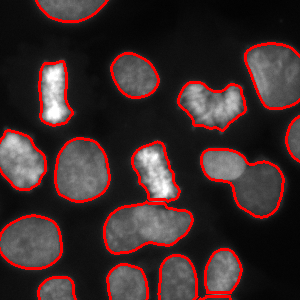
\includegraphics[width=37.5pt,height=37.5pt]{img/overlay.png}};
\draw (69,162) node  {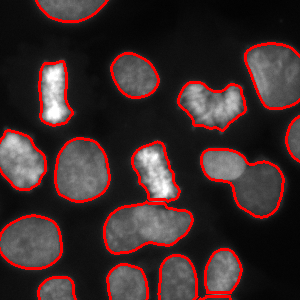
\includegraphics[width=56.25pt,height=56.25pt]{img/overlay.png}};
%Shape: Rectangle [id:dp2951489537408193] 
\draw   (124,137) -- (174,137) -- (174,187) -- (124,187) -- cycle ;

% Text Node
\draw (309,162) node [scale=7.5]  {$\Sigma $};
% Text Node
\draw (69,202.75) node [scale=0.7] [align=left] {Measurement unit};
% Text Node
\draw (149.5,203.5) node [scale=0.7] [align=left] {Feature representation};
% Text Node
\draw (229,203.5) node [scale=0.7] [align=left] {Dimensionality reduction};
% Text Node
\draw (309.5,203.5) node [scale=0.7] [align=left] {Aggregation strategy};

\end{tikzpicture}

\caption{A conventional high content analysis follows four ordered stages. Each stage may be accomplished by a variety of algorithms, and some stages may be omitted in certain pipelines, or subsumed to a common framework.}
\label{fig:intro_profiling}
\end{figure}

% \footnote{Some reminders: a metric is a distance function defined on a set of points. It satisfies the four properties: non-negativity, identify, symmetry, and the triangle inequality. A metric and set of points constitute a \emph{metric space}, and the metric induces a certain \emph{topology} on the set of points. A \emph{manifold} is a space that is locally homeomorphic to Euclidean space, for example a sphere. Recall a geodesic is the equivalent of a straight line on curved spaces, for example, the ``great circles'' on the surface of a sphere. A Reimannian manifold is a manifold endowed with additional properties. Topological spaces generalise metric spaces and manifolds. Geometries are systems founded on axioms of shapes. Euclidean geometry was the original geometry, characterised by five properties. Euclidean geometry is part of a broader system articulated in the \emph{Elements}, which is foundational to all of mathematics. The Cartesian plane, which assigns a pair of coordinates to every point in the two-dimensional Euclidean plane, unified geometry and algebra, revolutionising mathematics in the 17th century. Non-Euclidean geometries occur when the fifth postulate on parallel lines is relaxed, producing either hyperbolic or elliptical geometry. The former allows infinitely many non-intersecting non-parallel lines, and the latter allows none. Hyperbolic geometry, for example, is the geometry of a saddle surface--a surface with at least one saddle point (a stationary point that is, for example a local minima in one axis and local maxima in another).}

The measurement unit for high content analysis is by convention the cell (\cite{perlman2004multidimensional}, \cite{adams2006compound}), entailing a segmentation of the image. However, \emph{segmentation-free} direct analysis of the full image (\cite{orlov2008wnd}, \cite{uhlmann2016cp}), or image segments, have proven successful, in particular through application of deep learning (\cite{kraus2016classifying}). The tradeoff is between a fine-grained analysis at the cellular level, where careful consideration of cell structure and fluorescent colocalisation is a focus (\cite{slack2008characterizing}), and a coarse analysis of the cell population, where population densities and dynamics can be measured. Attempts to benefit from both scales have been made (\cite{godinez2017multi}). Our focus in Chapters \ref{Chapter2} and \ref{Chapter3} is individual, \emph{per cell} analysis. We detail our approach to segmentation of TNBC cells in Chapter \ref{Chapter2}.

Cell phenotypes are compiled through feature extraction of the measured unit. The features extracted are decided by the nature of analysis. We define three modes of high content analysis, in order of complexity:

\begin{itemize}
\item[I] \textbf{Univariate}: In the ideal case, biological functions may be quantitatively described by a single feature. For example, the nuclear area might increase dramatically under certain treatments. Thus, it would be sufficient to measure the corresponding feature (nuclear size) and statistically analyse its distribution for the different experimental conditions. Such a scenario would likely be easier to explain in biological terms.
\item[II] \textbf{Multivariate}: A more complex case arises when we analyse different phenotypic descriptors (biologically meaningful features) and their interdependencies. Then we would contend with the multi-variate distribution of these features, and our analysis would be necessarily more sophisticated.
\item[III] \textbf{Machine learning}: In a final case, phenotypes might not be discernible in such basic terms, and would would rather require the tools of statistical learning to elucidate the patterns in the cell population. In this case, we would rather extract a large number of features without clear biological meaning. Learning can then be unsupervised or supervised. In the supervised case, the biological meaning could be injected (by the analyst) through use of biologically meaningful classes.
\end{itemize}

In Chapter \ref{Chapter2} we develop a use case of each of these analysis types. The conventional line for a type III analysis is to extract some large number of plausibly discriminative image analysis features from the region of interest (RoI) of each segmented cell. These may include intensity, shape, textural, and statistical features, though their suitability will vary by fluorescent channel and the cell component imaged. A more modern alternative is to learn a feature extraction directly from the RoI pixels within the hidden layers of a neural network. We explore this alternative primarily in Part \ref{partII}, where the presence of fluorescence marker alone is enough to classify the cell phenotype.

Dimensionality reduction is usually a component of a type III analysis. Here, the options abound, and a comparison of approaches is a primary focus of Chapter \ref{Chapter3}. The choice of approach is determined by the analytical objectives. In the simple case of counting cell class, a classifier of cell types such as in \cite{neumann2010phenotypic}, and which we explore in Chapters \ref{Chapter2} and \ref{Chapter4}, performs the role of dimensionality reduction: the classifier maps the feature vector of each cell to a scalar or one-hot encoding representing cell class.

\begin{equation}
f : \mathbf{x} \to \{0, 1\}^K
\end{equation}

The cell population is then summarised in $\mathbf{p} \in \mathbf{R}^K$, obtained by aggregation as a simple summation or average, giving the number or proportion of cells per cell class respectively,

\begin{equation}
\mathbf{p} = \frac{1}{N}\sum_{i=1}^N f(\mathbf{x}_i)
\end{equation}

for the $N$ cells in the population. In a more complex case, we reduce the features to a vector of obscure indices (for example, a set of principal components derived over the population of cell feature vectors). The \emph{phenotypic profile}, a signature characterising the effect of a drug on the cell population (see Chapter \ref{Chapter3}), may be set to the population centroid (as in \cite{adams2006compound}), or otherwise more sophisticated aggregation algorithms exist such as in \cite{perlman2004multidimensional} and \cite{loo2007image}. Though useful as the basis of comparison in drug screens and elsewhere, aggregated phenotypic profiles lose distributional information (\cite{altschuler2010cellular}), as a multi-modal populations may be reduced to unrepresentative centroids. This problem is potentially exacerbated in multi-cell-line data, a problem we address in Chapter \ref{Chapter3}.

In applications of deep learning, a neural network may perform several of the Figure \ref{fig:intro_profiling} stages simultaneously, as neural networks naturally incorporate feature extraction and dimensionality reduction components (\cite{sommer2017deep}). Indeed, segmentation may also be included as a byproduct of neural object detection (see Appendix \ref{AppendixA}). Thus, we succeed in incorporating all stages of the pipeline into a convolutional neural network in Chapter \ref{Chapter4}.

\section{Challenges for high content analysis}

High content analysis offers many interesting research directions. Those most relevant to this dissertation are described in the following.

\subsection{Heterogeneous cell line data}

As mentioned above, a single cell line may be a flawed or incomplete model for a disease. This motivates the validation of discoveries against multiple cell lines, representing different subtypes of the same disease. It is furthermore a step in the direction of the emerging paradigm of precision medicine (\cite{ashley2016towards}), where machine learning will play a decisive role (see, for example, \cite{krittanawong2017artificial}). Genomics has led the way so far, but other data sources including images are expected to be increasingly part of the picture \cite{hulsen2019big}. Quantifying drug effects with respect to multiple cell lines allows to identify cell-line-specific drug effects against unilateral effects. A multi-cell line screen, where several cell lines representative of a common disease are subjected to the same set of perturbations, is therefore well motivated. Such is the aim of Part \ref{partI}, which screens multiple triple negative breast cancer (TNBC) cell lines.

\begin{figure}%
    \centering
    \subfloat[MDA231]{{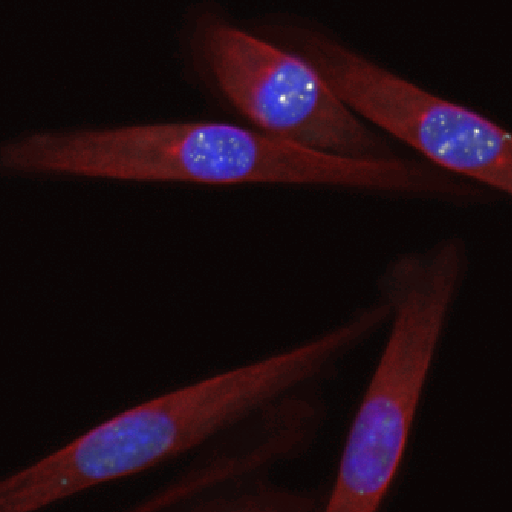
\includegraphics[width=0.45\textwidth]{img/mda231_morphologies.png}}}
    \qquad
    \subfloat[MDA468]{{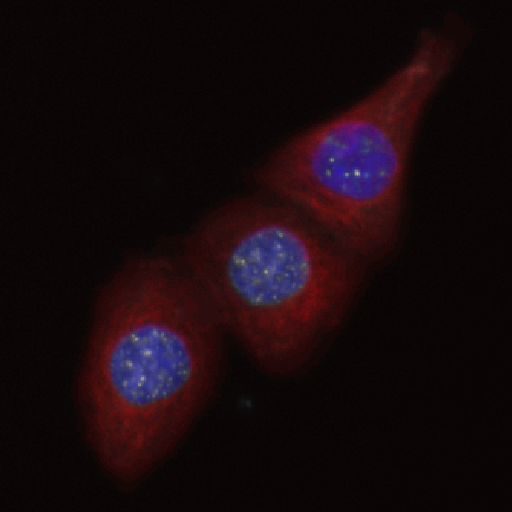
\includegraphics[width=0.45\textwidth]{img/mda468_morphologies.png}}}
	\caption{Comparison of cells sampled from negative control wells containing a) TNBC cell line MDA231 and b) TNBC cell line MDA468. Cell nuclei appear in blue, cell microtubules appear in red.}
    \label{fig:cell_line_morphologies}%
\end{figure}

However, such a screen creates a heterogeneity of data. For example, TNBC cell lines MDA231 and MDA468 manifest different morphologies, in their unperturbed state. Figure \ref{fig:cell_line_morphologies} shows samples of cells taken from microplate wells containing negative control dimethyl sulfoxide (DMSO). The cells are imaged with the same set of fluorescent markers. One observes clear differences in these archetypal morphologies, with MDA231 cell exhibiting nuclei and cytoskeleton, compared to isotropic MDA468 cells. This has second-order effects such as the degree of geometric tessellation   between groups of cells. Combining multi-cell-line data  has been addressed by different approaches by \cite{rose2018compound} and \cite{warchal2016development}. In Chapter \ref{Chapter3} we propose and evaluate a new method for addressing this problem by modeling the heterogeneous datasets as divergent feature domains requiring adaptation. Cells from the divergent domains are mapped to a \emph{domain-invariant} feature space by an adversarial neural network training strategy (\cite{ajakan2014domain}).

\subsection{The emergent role of deep learning in high content screening}

Deep learning is touted as a panacea for computer vision problems, and high content data ought not to be an exception. However, the successful deployment of deep neural networks relies crucially on vast volumes of data to enable effective generalisation. Large annotated datasets such as ImageNet (\cite{russakovsky2015imagenet}) were one of a few key preconditions that fostered the rise of deep learning for object classification in 2012 (we give a brief history in Appendix \ref{AppendixA}), and extensions of deep learning to other problem domains were likewise accompanied by the curation of large, special-purpose datasets, for example \cite{lin2014microsoft} for object detection. However, annotated data for supervised training is expensive, requiring manual effort, often by domain experts. ImageNet leverages online crowdsourcing platforms (quality is ensured by the consensus of multiple annotators). This is a bottleneck for all deep learning research, and therefore extends to computational phenotyping. The Broad Institute benchmark collection (BBBC) datasets (\cite{ljosa2012annotated} and, specifically, \cite{caie2010high}) have become a sort of benchmark for developing drug response phenotyping algorithms (for example, \cite{kraus2016classifying} or \cite{kandaswamy2016high}).

Nevertheless, in recent years, a significant trend in deep learning research has been on making better use of available data. After all, even if annotated data is hard to come by, unlabeled or \emph{weakly labeled} is available in abundance. For example, \cite{mahajan2018exploring} used $3.5$ billion social media images ``weakly annotated'' with hashtags to pretrain a state-of-the-art system for object classification. Indeed, notable applications of deep learning in HCS thus far have relied on weakly supervised learning \cite{kraus2016classifying}, \cite{godinez2017multi}. Elsewhere, contrastive learning (for example, \cite{chen2020simple}) may yet revolutionise the training of deep learning systems by making more efficient use of data, achieving parity with state-of-the-art systems with only a small faction of data.

A recent trend in bioimage analysis has been the prediction of one mode of microscopy from another. Microscopes with the capacity of registering multiple modes of microscopy simultaneously, for example transmitted light and fluorescence images, automatically create an image-to-image translation dataset. Fluorescence labeling as a pixel-wise regression problem has been successfully demonstrated by \cite{christiansen2018silico} and \cite{ounkomol2018label}, where deep multi-task neural networks are furthermore capable of labeling multiple independent fluorescent channels simultaneously. Earlier, \cite{sadanandan2017automated} used fluorescence to construct cell segmentation datasets automatically. These works have shown how one may exploit imaging protocols to bypass the manual annotation bottleneck for deep learning. We explore this possibility in Chapter \ref{Chapter4}, contrasting two approaches for leveraging fluorescence as an automatic annotator.

Generative models represent another trend in computer vision (\cite{kingma2013auto}, \cite{goodfellow2014explaining}, \cite{oord2016pixel}), modeling the marginal distribution on data, allowing for data synthesis, in particular image synthesis. Generative adversarial networks (GANs) (\cite{goodfellow2014explaining}) are the most highly developed of deep generative models, and have already found use in high content image data (for example, in \cite{osokin2017gans}). In Part \ref{partII} GANs feature heavily in several use cases.

%\section{Software}
%
%The development of the research underpinning this dissertation is greatly indebted to the open-source software listed below, with which the vast majority of image processing, machine learning analysis, and visualisations were. The usage of other software will be cited throughout the text.
%
%\subsection{Cell Cognition}
%
%Cell Cognition (\cite{held2010cellcognition}) is an open-source software for the visualisation and analysis of high content screening assays, and is a collaborative project between the CBIO and the Gerlich group at the IMBA in Vienna. In our reserach, Cell Cognition is used, for data inspection, feature extraction, annotation, and model training. The starting point for most of the following analyses is to extract a large number of morphological and textural features from the image data with Cell Cognition. Cell Cognition first segments the nuclei (on the DAPI channel), a result that can be used to segment further on the other channels, for example Cy5, in order to segment the cell membrane. Features may then be calculated at the \emph{per-cell} level for the entire population of the assay. As a HCS analysis tool, Cell Cognition competes with CellProfiler (\cite{lamprecht2007cellprofiler}).
%
%\subsection{Python}
%
%\texttt{Python} is a scripting language that dominates applications in data science. Below we list the most important frameworks.
%
%\subsubsection{Jupyter}
%
%Jupyter is an open-source project (based on the earlier IPython) that provides an interactive \textsc{Python}\footnote{Jupyter supports other scripting languages too, such as \textsc{R} and \textsc{Julia}.} shell called a \emph{notebook} that runs through a web browser. Organised into a sequence of executable \emph{cells}, a Jupyter notebook provides the user with a persistent environment for writing code, markdown (supporting \TeX), and rich media into a presentable and portable document format. From an architectural standpoint, Jupyter notebooks are designed for showcasing the outputs of code modules, which may be imported into the environment. Jupyter is particularly useful as a ``sandbox'', where code snippets can be tested rapidly. For these reasons, Jupyter is favoured as a tool for \emph{reproducible research} (\cite{kluyver2016jupyter}), alongside others such as \textsc{R Markdown}. It is certain that more notebook tools will emerge in the years to come, with trends in collaborative notebooks and notebook-based articles already in motion. We use Jupyter extensively in our analysis.
%
%\subsubsection{Keras}
%
%\texttt{Keras} (\cite{chollet2015keras}) is a wrapper library for \texttt{TensorFlow} (\cite{tensorflow2015-whitepaper}), \texttt{Theano} (\cite{2016arXiv160502688full}), and other core frameworks. It is perhaps unmatched for assembling and training basic neural networks quickly, yet it embodies the declarative nature of its framework backends. It is therefore often difficult to debug, and flies in the face of the interpreted nature of \texttt{Python}.
%
%\subsubsection{Pytorch}
%
%\texttt{PyTorch} (\cite{paszke2017automatic}) is the result of merging the \texttt{Torch} and \texttt{Caffe} projects, curated by the Facebook corporation. \texttt{PyTorch} is in its own right a powerful tool for analysis, roughly amounting to a GPU-accelerated \texttt{NumPy} (\cite{numpy}). The \emph{autograd} package permits differentiable computational graphs to be invoked on-the-fly, and a neural network sub-library predefines a wide array of flexible \emph{modules} apt for neural network building. Though requiring more boilerplate code than \texttt{Keras}, typical workflows are vastly more readable and workable.

\section{Contributions}

This dissertation encompasses work completed on two unique projects in high content analysis. It is therefore organised into two parts, each containing two chapters. The two parts can be read in any order, but they internally follow a progression of ideas that are intended to be read in order of appearance. Each chapter is oriented around a published paper, with the exception of the final chapter, which follows a work in progress.

Part \ref{partI}, comprising of Chapters \ref{Chapter2} and \ref{Chapter3} covers our drug screen of multiple TNBC cell lines. Chapter \ref{Chapter2} is introductory and aims to describe the workflows of high content screening and its modes of analysis, while following examples from our drug screen, including the multivariate analysis on \emph{double strand break} detection, published in the proceedings of ISBI 2018 (\cite{boyd2018analysing}) (which we include in Appendix \ref{AppendixD}. It concludes with a pair of case studies on \emph{phenotypic profiling}, that are intended to dovetail into \emph{Chapter 3}, which serves as a review of profiling methodologies, and develops a new profiling approach for multiple cell lines. This approach is to combine heterogeneous data from different cell lines using domain adaptation. The chapter is an extended version of our paper published in the journal Bioinformatics (\cite{boyd2020domain}). We additionally released the dataset for this project, to our knowledge, the first of publicly available dataset of its kind (\cite{Boyd_Reyal_Pinheiro_Del_Nery_Walter_2019}) alongside an open source code repository including worked, reproducible workflows\footnote{https://github.com/jcboyd/multi-cell-line}.

Part \ref{partII}, comprising of Chapters \ref{Chapter4} and \ref{Chapter5} covers our CAR-T experiments. Chapter \ref{Chapter4} compares two approaches to utilising fluorescence microscopy as an automatic annotator of paired phase contrast microscopy. The second of the two approaches, based on a customised object detection system, was published in the proceedings of ISBI 2020. We again made our datasets public (\cite{Boyd_Gouveia_Perez_Walter_2019}) as well as source code and scripts for reproducible experiments\footnote{https://github.com/jcboyd/detecting-lymphocytes}.  A modified version of this paper is included inline. Finally, the shortcomings of the two approaches are reconsidered in Chapter \ref{Chapter5}, and a creative alternative solution is proposed, based on data augmentation by image synthesis using generative models. The final section of the chapter is intended as a template for a future publication. 

Not included in this dissertation are minor contributions made as a second author to a study on predicting residual cancer burden from TNBC histopathology images, published in the proceedings of ISBI 2019 (\cite{naylor2019predicting}), and an as-of-yet unpublished paper on a new structured dropout algorithm for regularising neural networks \cite{khalfaoui2019adaptive}.

